\section{Introduction}

The recent emergence of popular omnidirectional cameras and Head-Mounted-Displays (HMDs) has increased the amount of 360-video content available \cite{mendes_2020}. Omnidirectional videos are spherical visual signals that allow the viewer to look around a full 360-degree view of a scene from a specific point. When using HMDs, at each instant in time, the viewer is presented with a viewport that is updated as the viewer moves their head. This type of content, especially when consumed through Virtual Reality~(VR) devices (HMDs included), can provide immersive experiences in which the user has a strong feeling of presence when compared with the use of traditional media \cite{montagud_culture_2020}.

Several people use subtitles when consuming audiovisual media, and these subtitles are important in contributing to the understanding of the video content \cite{brown_subtitles_2017}. There are even people who choose to consume videos without the sound turned on \cite{hughes_disruptive_2019}. Additionally, the work of \citeonline{hayati2011effect}, as referenced in \citeonline{hughes_disruptive_2019}, shows that consumers are more likely to watch videos entirely if they have subtitles presented with them. In traditional 2D videos, static subtitles are commonly used and they are usually placed at the center-bottom of the screen \cite{rothe_dynamic_2018}.

Different from traditional 2D videos, subtitles positioning in 360-videos is challenging because it involves both temporal and spatial domains \cite{agullo2019making}, and there is no ``center-bottom" of the screen in a 360-video \cite{brown_subtitles_2017}. Most current solutions rely on positioning subtitles either statically to the viewer or at a fixed position in the 360-degree environment \cite{mendes_2020}. According to \citeonline{li_impacts_2018}, in a journalistic 360-videos case study, the subtitles viewing behaviour is dependent on the type of content. 

Equirectangular projection is the most common way for representing and transmitting 360° video~\cite{yang2018object}. With the equirectangular projection, each sphere point is defined by two angles~\cite{snyder1987map}: \emph{latitude}~$\theta \in [-90^{\circ}, +90^{\circ}]$ and \emph{longitude}~$\phi \in [-180^{\circ}, +180^{\circ}]$. This kind of projection creates challenges for image processing and computer vision algorithms, especially to the convolution-based ones because of the severe distortions in areas vertically distant from the center of the image~(see Figure \ref{fig:equirectangular_proj}).

\begin{figure}[!ht]
\centering
    \begin{subfigure}{0.47\linewidth}
        \centering
        
\includegraphics[width=1\textwidth]{img/image (9).jpg}
        \caption{Outdoor equirectangular image.}
        \label{subfig:out_equi}
    \end{subfigure}\hfill
    \begin{subfigure}{0.47\linewidth}
        \centering
        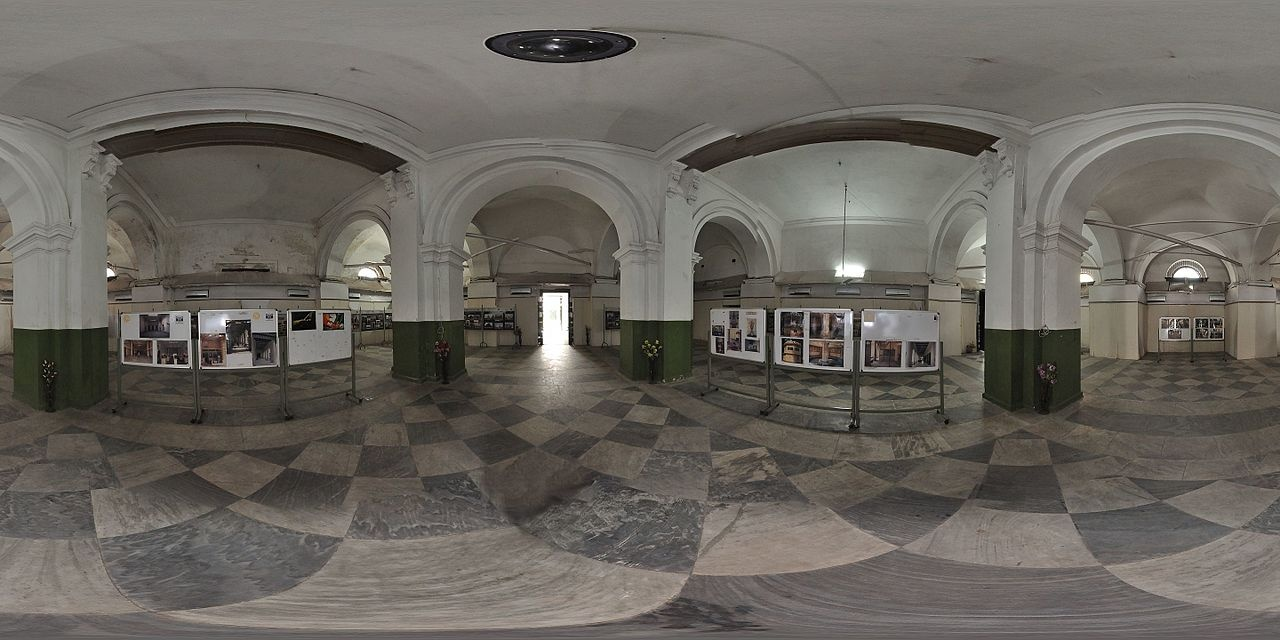
\includegraphics[width=1\textwidth]{img/image (10).JPG}
        \caption{Indoor equirectangular image.}
        \label{subfig:in_equi}
    \end{subfigure}

\caption{Examples of 360° scenes represented through equirectangular projection.}
\label{fig:equirectangular_proj}
\end{figure}

The remainder of this dissertation proposal is structured as follows. Section~\ref{sec:subtitles} presents the current solutions for subtitles positioning in 360º video. Section~\ref{sec:approach} details our approach for automatic subtitles positioning. Finally, Section~\ref{sec_4} presents some final considerations such as the current status of our work, the next steps, and the work schedule.